\documentclass[10pt]{beamer}

\usepackage[czech]{babel}
\usepackage[utf8]{inputenc}

\usetheme{metropolis}
\usepackage{appendixnumberbeamer}

\usepackage{booktabs}
\usepackage[scale=2]{ccicons}

\usepackage{subfig}
\usepackage{multicol}

% tables and cline
\usepackage{makecell}
\usepackage{multirow}
\usepackage{regexpatch}
\makeatletter
% Change the `-` delimiter to an active character
\xpatchparametertext\@@@cmidrule{-}{\cA-}{}{}
\xpatchparametertext\@cline{-}{\cA-}{}{}
\makeatother

\usepackage{xspace}
\newcommand{\themename}{\textbf{\textsc{metropolis}}\xspace}

\title{Rozpoznávání fonémů pomocí neuronových sítí}
\author{Martin Majer}
\date{}
\institute{Katedra kybernetiky\\Fakulta aplikovaných věd\\ Západočeská univerzita v Plzni}

\begin{document}

\maketitle

\begin{frame}{Úvod do problematiky a cíle práce}
	\begin{itemize}
		\item porovnání různých typů neuronových sítí a parametrizací řečového signálu pro úlohu rozpoznávání fonémů		
		\item porovnáváno na dvou datových sadách v českém jazyce:
			\begin{itemize}
				\item ŠkodaAuto - 47 řečníků, 14523 nahrávek
				\item SpeechDat-E - 924 řečníků, 39560 nahrávek
			\end{itemize}
		\item foném = základní fonologická jednotka, která se definuje jako nejmenší lingvistická jednotka schopná rozlišovat významové jednotky (slova)
		\item rozpoznávání fonémů = úloha, jejíž cílem je pro danou zvukovou nahrávku získat odpovídající sekvenci fonémů
	\end{itemize}
\end{frame}

\begin{frame}{Typy příznaků}
	\begin{itemize}
		\item využity příznaky ve frekvenční oblasti:
			\begin{itemize}
				\item logaritmované energie banky filtrů
				\item mel-frekvenční kepstrální koeficienty
			\end{itemize}
		\item využití Z-score normalizace
			\begin{align*}
				z = \dfrac{x - \mu}{\sigma}
			\end{align*}
		\item využití delta a delta-delta koeficientů
	\end{itemize}
\end{frame}

\begin{frame}{Typy neuronových sítí}
	\begin{itemize}
		\item využité typy neuronových sítí:
			\begin{itemize}
				\item dopředná neuronová síť s Viterbiho dekodérem
				\item LSTM/GRU/obousměrná LSTM s Viterbiho dekodérem
				\item LSTM/obousměrná LSTM s CTC
			\end{itemize}
		\item Viterbiho dekodér využívá zerogramový jazykový model
		\item využita metoda předčasného ukončení a zašumění trénovacích dat Gaussovským šumem
	\end{itemize}
\end{frame}

\begin{frame}{Rekurentní neuronová síť - schéma}
	\begin{figure}
		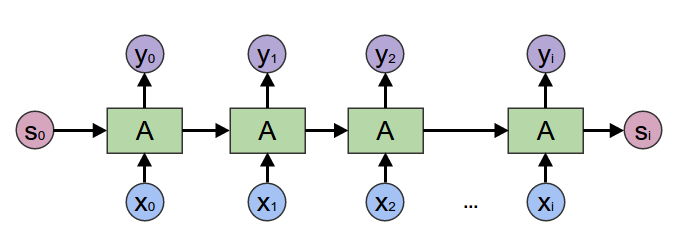
\includegraphics[width= 0.8\linewidth]{rnn_general.png}
	\end{figure}
	
	\begin{figure}
		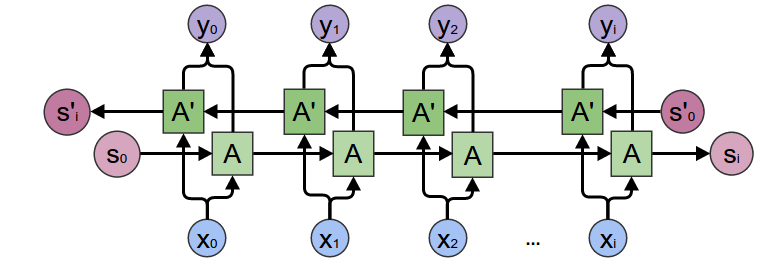
\includegraphics[width= 0.8\linewidth]{rnn_bidirectional.png}
	\end{figure}
	
	Převzato z \textit{http://colah.github.io/posts/2015-09-NN-Types-FP}
\end{frame}

\begin{frame}{LSTM - schéma}
	\begin{figure}
		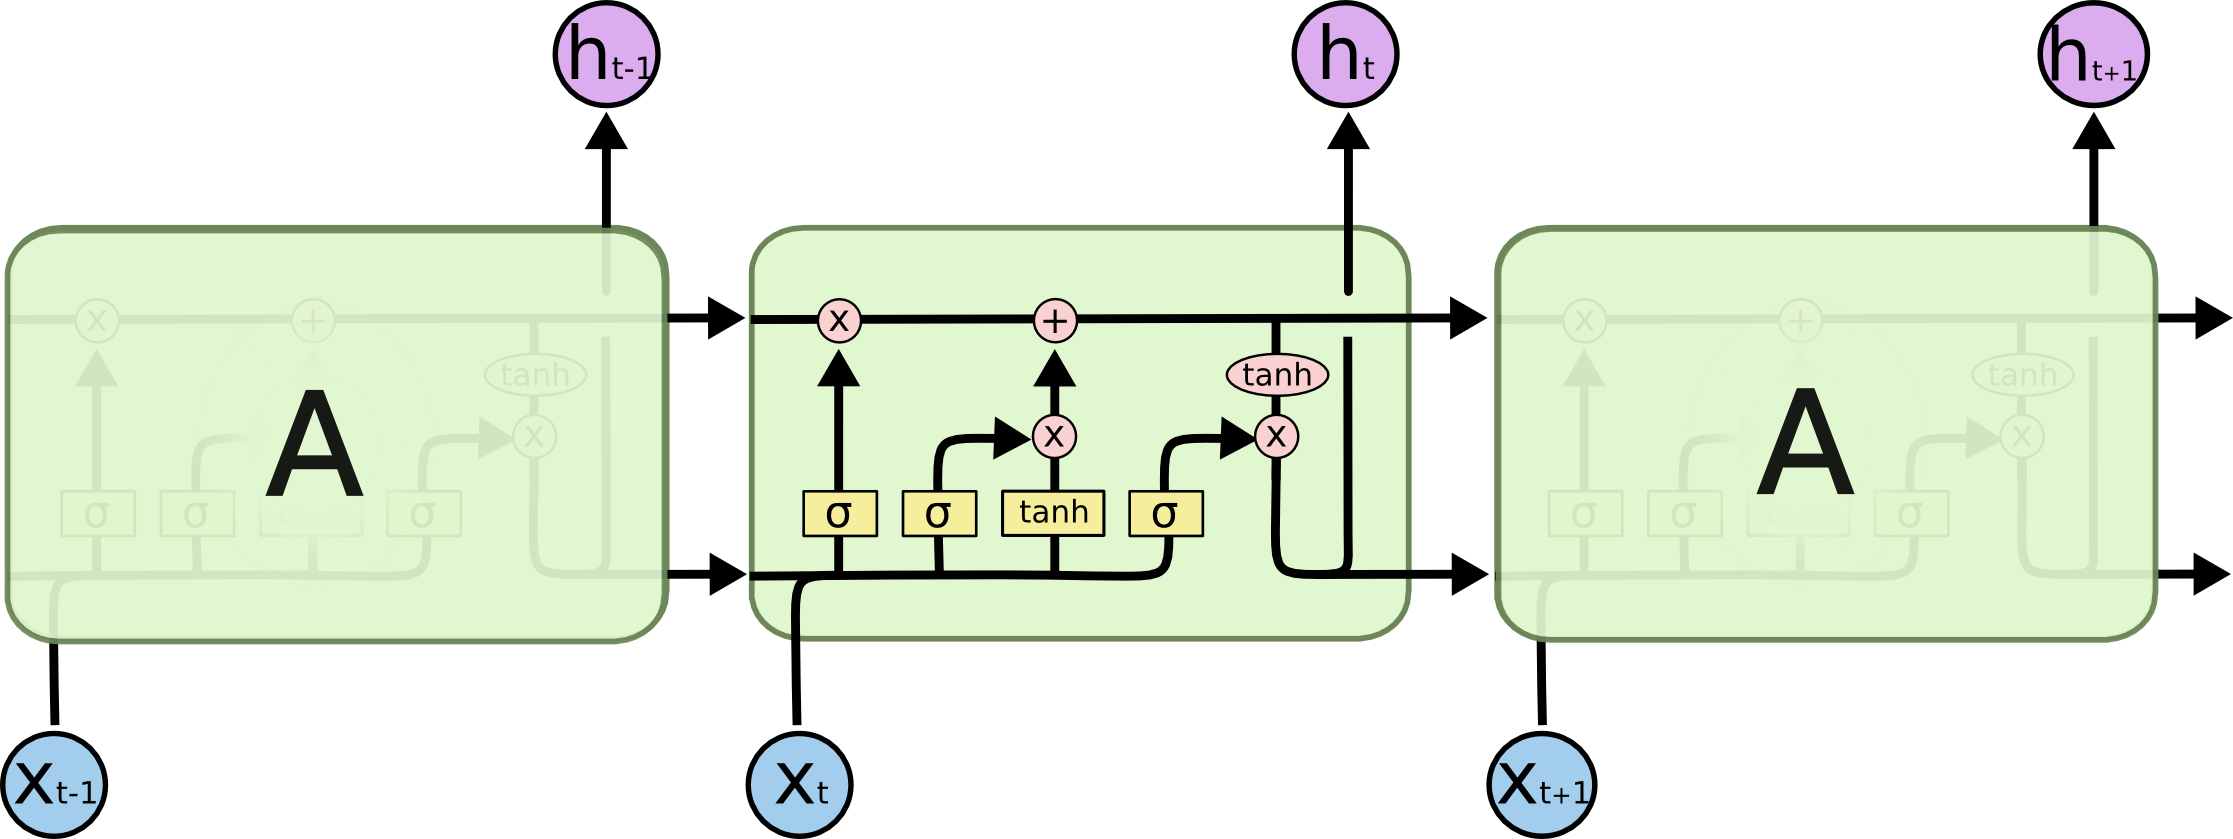
\includegraphics[width= 0.8\linewidth]{lstm.png}
	\end{figure}
	
	\centering	
	Převzato z \textit{http://colah.github.io/posts/2015-08-Understanding-LSTMs}
\end{frame}

\begin{frame}{CTC (connectionist temporal classification)}
	\begin{itemize}
		\item není potřeba segmentovat nahrávky po fonémech
		\item není potřeba dále zpracovávat výstup sítě
		\item hledáme nejpravděpodobnější značkování $ l $ pro vstupní obraz $ x $, tj. $ argmax \text{ } p(l \mid x) \rightarrow $ zavedení prázdného znaku a využití dopředného a~zpětného algoritmu 
		\item využito dekódování nejlepší cesty bez jazykového modelu
	\end{itemize}
\end{frame}

\begin{frame}{CTC - schéma}
	\begin{figure}
		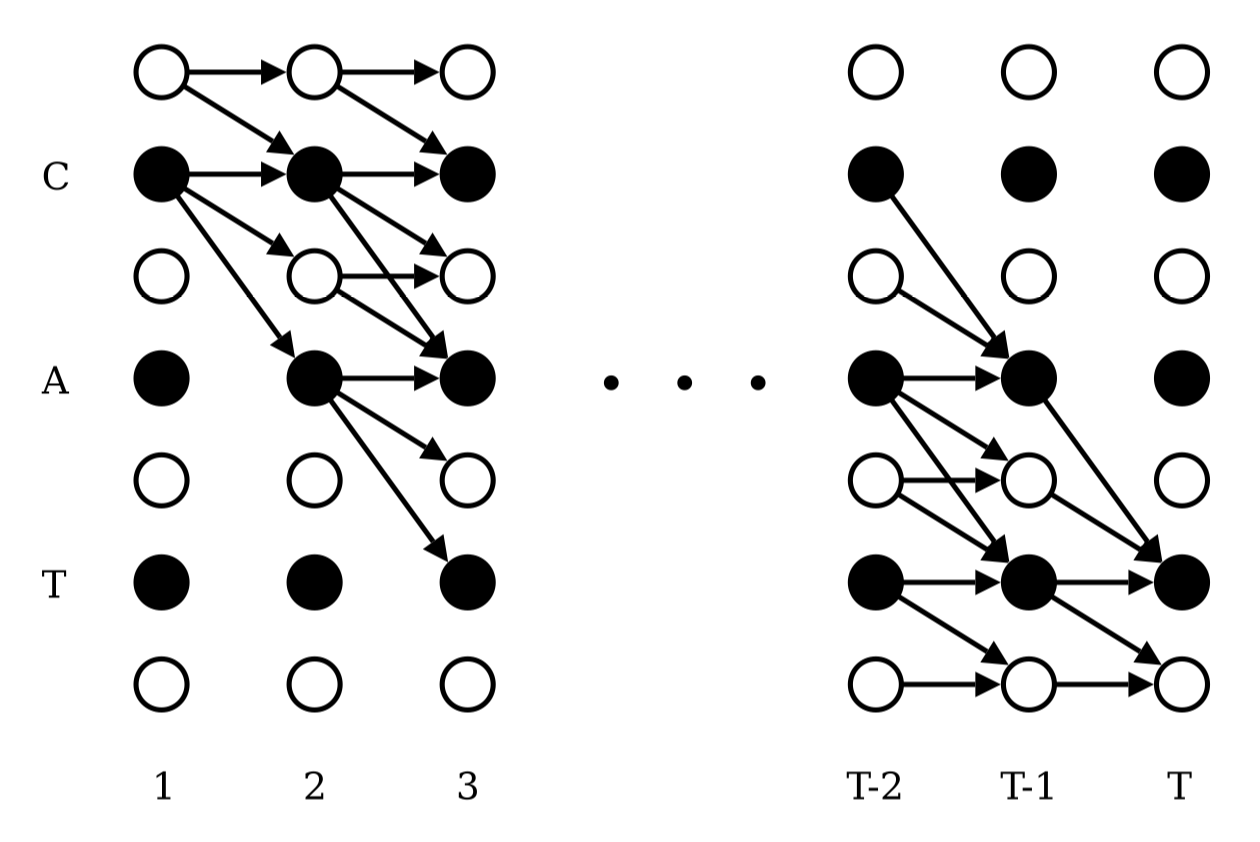
\includegraphics[width= 0.8\linewidth]{ctc.png}
	\end{figure}
	
	\centering
	Převzato z \textit{Connectionist Temporal Classification: Labelling Unsegmented Sequence Data with Recurrent Neural Networks, A. Graves, 2006}
\end{frame}

\begin{frame}{Vyhodnocení}
	\begin{itemize}
		\item hlavní vyhodnocovací metrika:
			\begin{itemize}
				\item \textbf{phoneAcc [\%]} - přesnost modelu po dekódování
					\begin{align*}
						\text{phoneAcc } = \dfrac{phones \text{ } correct - phones \text{ } inserted}{phones \text{ } total} \cdot 100
					\end{align*}
			\end{itemize}
		\item další zohledněné metriky:
			\begin{itemize}
				\item \textbf{frameAcc [\%]} - přesnost klasifikace modelu vyhodnocována po jednotlivých segmentech nahrávek
				\item \textbf{phoneCorr [\%]} - procento správně klasifikovaných fonémů po dekódování
			\end{itemize}
	\end{itemize}
\end{frame}

\begin{frame}{Vyhodnocení}
	\begin{table}[H]
		\centering
		\resizebox{1.0\textwidth}{!}{\begin{tabular}{ |c|c|c|c|c|c|c|c|c| }
			\cline{2-9}
			\multicolumn{1}{c}{} & \multicolumn{4}{|c|}{ŠkodaAuto} & \multicolumn{4}{c|}{SpeechDat-E} \\
			\hline
			architektura & LFE & \makecell{LFE \\ $ \Delta\Delta$} & MFCC &  \makecell{MFCC \\ $ \Delta\Delta$} & LFE &  \makecell{LFE \\ $ \Delta\Delta$} & MFCC &  \makecell{MFCC \\ $ \Delta\Delta$} \\
			\hline
			dopředná & 79.99 & 80.15 & 79.63 & 81.06 & 68.65 & - & 68.92 & 69.88 \\
			\hline
			LSTM & 76.45 & 78.17 & 67.10 & 79.56 & - & - & 62.87 & 68.80 \\
			\hline
			GRU & 72.84 & 73.49 & 73.12 & 77.65 & - & - & 59.86 & 65.53 \\
			\hline
			obousměrná CTC LSTM & 92.97 & 93.34 & 93.03 & 93.70 & 81.22 & 82.11 & 80.42 & 83.23 \\
			\hline
			dávková CTC LSTM & 63.04 & 68.58 & 65.28 & 70.80 & 58.32 & 60.87 & 60.05 & 63.81 \\
			\hline
			\makecell{obousměrná \\ dávková CTC LSTM} & 72.31 & 72.74 & 72.19 & 75.19 & 62.42 & 66.81 & 63.42 & 67.87 \\
			\hline
		\end{tabular}}
	\end{table}
	
	\centering
	Přesnost rozpoznávání po dekódování [\%]
\end{frame}

\begin{frame}{Vyhodnocení - ŠkodaAuto}
	\begin{figure}
		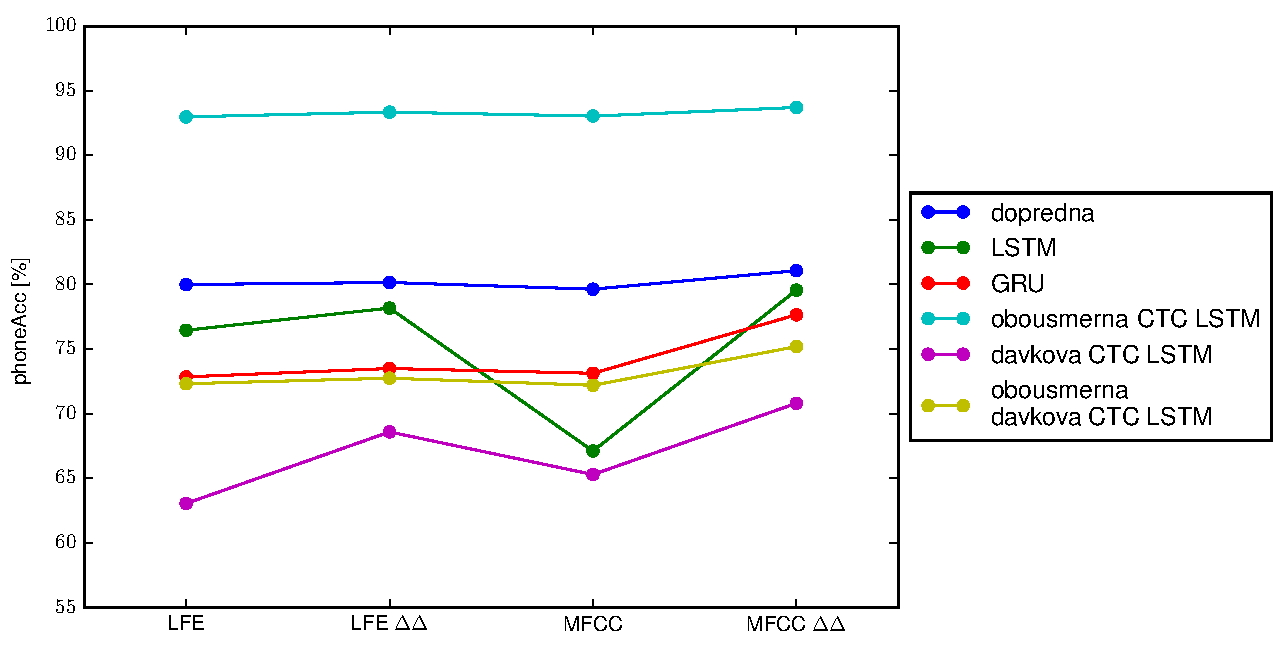
\includegraphics[width=1.0\linewidth]{skoda_results.pdf}
	\end{figure}
\end{frame}

\begin{frame}{Vyhodnocení - SpeechDat-E}
	\begin{figure}
		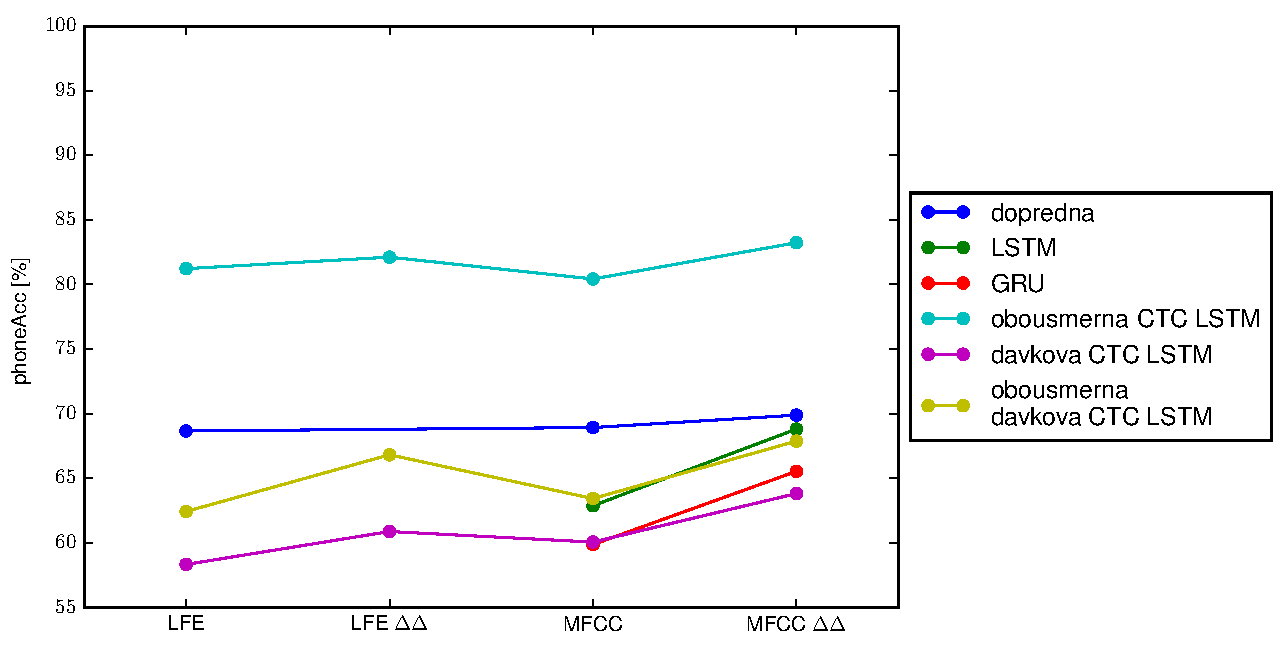
\includegraphics[width=1.0\linewidth]{speechdat_results.pdf}
	\end{figure}
\end{frame}

\begin{frame}{Shrnutí}
	\begin{itemize}
		\item navrženo a porovnáno šest architektur neuronových sítí
		\item akcelerační koeficienty zvyšují přesnost rozpoznávání
		\item nejvyšší přesnost rozpoznání pro obousměrnou LSTM síť s CTC
			\begin{itemize}
				\item přes 90\% na datové sadě ŠkodaAuto
				\item přes 80\% na datové sadě SpeechDat-E
			\end{itemize}
		\item rozpoznávání na základě znalosti celé nahrávky $ \rightarrow $ nevhodné pro rozpoznávání v reálné čase
		\item možná rozšíření práce:
			\begin{itemize}
				\item optimalizace topologie LSTM nebo dávkové obousměrné LSTM sítě s CTC
				\item nalezení kompromisu mezi velikostí sítě, délkou vstupní sekvence a dostatečnou přesností pro rozpoznávání v reálném čase
			\end{itemize}
	\end{itemize}
\end{frame}

\end{document}
